% !TeX root = main.tex

\subsection{Rule-based Constant time-scaling}

Say we have a time expression (function) $x(t)$. We first obtain $\dot{x}(t)$ by taking the time derivative $\dot{x}(t) = \sfrac{dx}{dt}$. 
We then obtain the time range within which this time scaling trick has to be applied. This could be obtained through a sensor. Say this time range is $t_{c1}$ and $t_{c2}$ (in the original time frame $t$).

We then find the new time values in the scaled time frame $\tau$ such that they are increased (farther apart), while the velocity $\dot{x}$ between them reduces. This is both related by the same constant $k$.

After scaling the velocity down by $k$ and scaling time $t_{c2}$ up by $k$, we resume the original velocity (as it was after the original $t_{c2}$). This marks the end of time scaling. However, the entire process will now end later (since the time between $t_{c1}$ and $t_{c2}$ was elongated). This concept is demonstrated in figure \ref{fig:cts-rb-holo}.

\begin{figure}[ht]
    \centering
    \begin{subfigure}[b]{0.4\textwidth}
        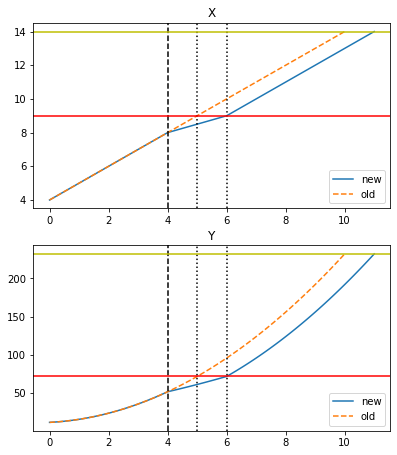
\includegraphics[width=\textwidth]{rb-cts-holo.png}
        \caption{Time scaling}
    \end{subfigure}
    \begin{subfigure}[b]{0.3\textwidth}
        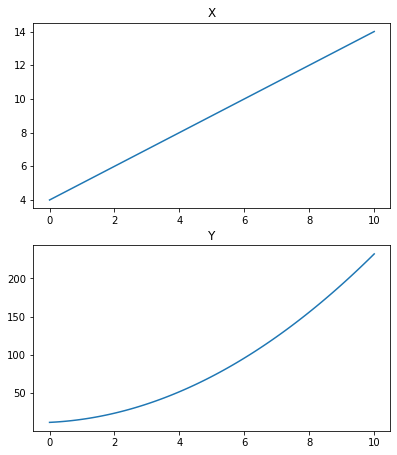
\includegraphics[width=\textwidth]{rb-cts-holo-origxy.png}
        \caption{Original}
    \end{subfigure}
    \begin{subfigure}[b]{0.25\textwidth}
        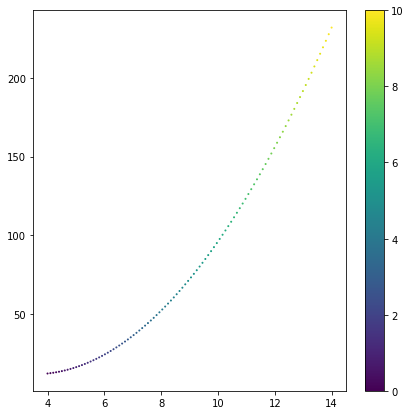
\includegraphics[width=\textwidth]{rb-cts-holo-xy.png}
        \caption{XY}
    \end{subfigure}
    \caption{Time scaling}
    \label{fig:cts-rb-holo}
    \small
        The variables $X$ and $Y$ are functions of time. The time scaling is applied from $4$ to $5$ seconds, with $k=0.5$ (the new end of time scaling will therefore happen at $6$ seconds).

        In left figure, it is apparent that the velocities have decreased to half in the time scaling period, while the duration has doubled.

        The center and right figures show the original trajectory ($X$ and $Y$ as function of time in center, and $X$ vs. $Y$ plot in the right).
\end{figure}

An example code implementing and testing this is available in appendix \ref{app:holo-rb-cts-code}. However, note that the code there implements time scaling on independent functions of time, and we are dealing with a constrained (non-holonomic) system.

We get around this by modelling the angle as $\theta = \textup{atan2} \left ( \dot{y},\dot{x} \right )$ along the entire new (time scaled) trajectory. The code for this is available in appendix \ref{app:nh-rb-cts-code}. The results from a simulation run are shown in figure \ref{fig:rb-cts-exp1}.

\begin{figure}[ht]
    \centering
    \begin{subfigure}[b]{0.3\textwidth}
        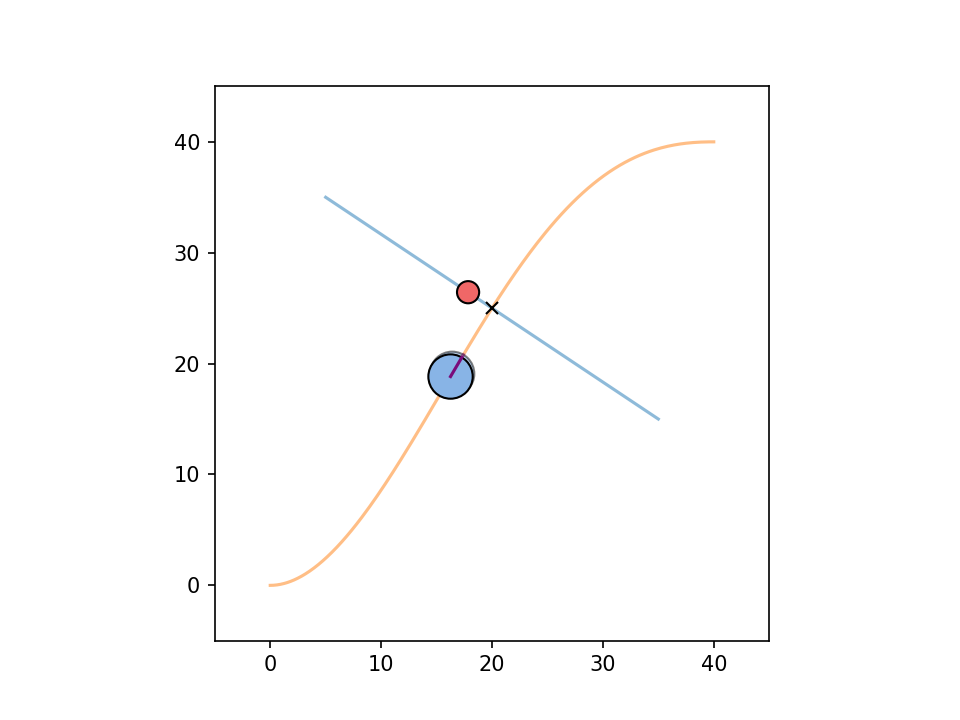
\includegraphics[width=\textwidth]{res1-ts-start.png}
        \caption{Start}
    \end{subfigure}
    \begin{subfigure}[b]{0.3\textwidth}
        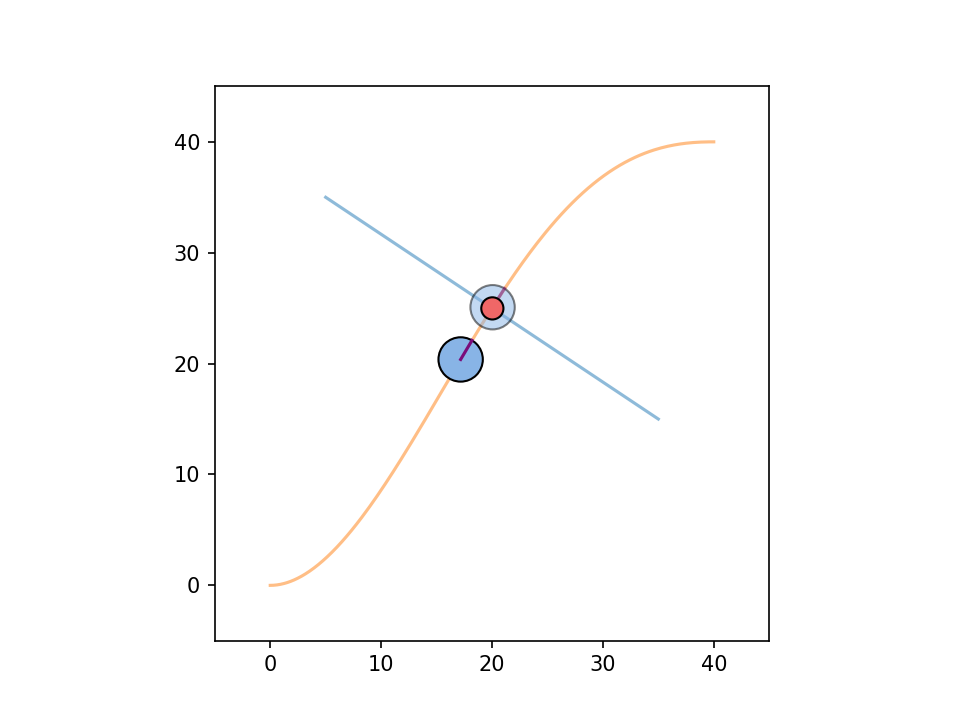
\includegraphics[width=\textwidth]{res1-ts-colav.png}
        \caption{Collision avoidance}
    \end{subfigure}
    \begin{subfigure}[b]{0.3\textwidth}
        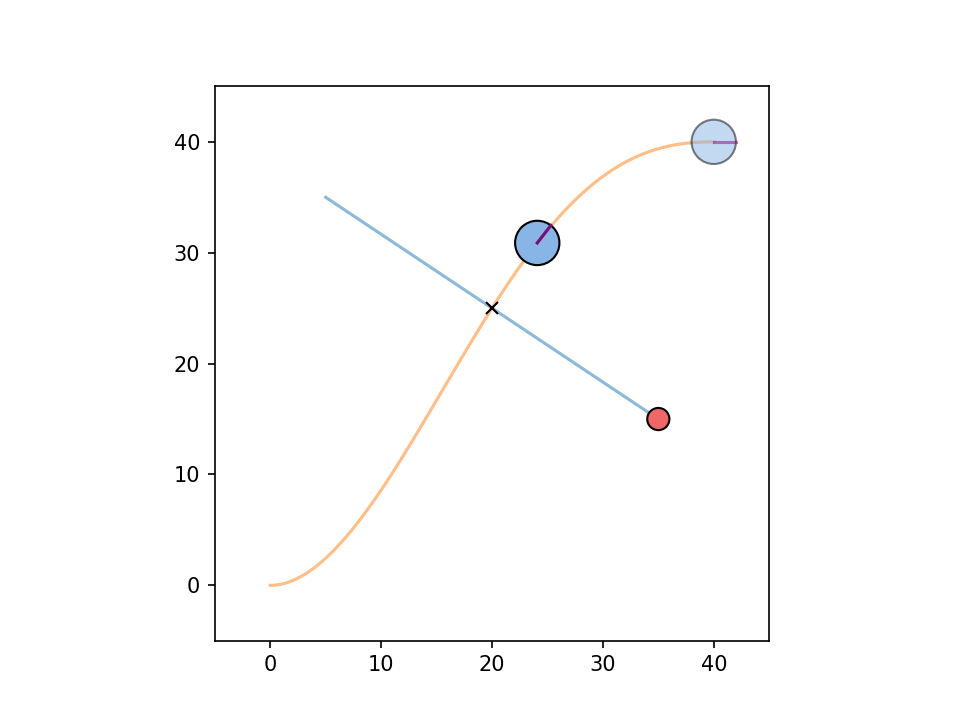
\includegraphics[width=\textwidth]{res1-ts-end.png}
        \caption{End}
    \end{subfigure}
    \begin{subfigure}[b]{0.45\textwidth}
        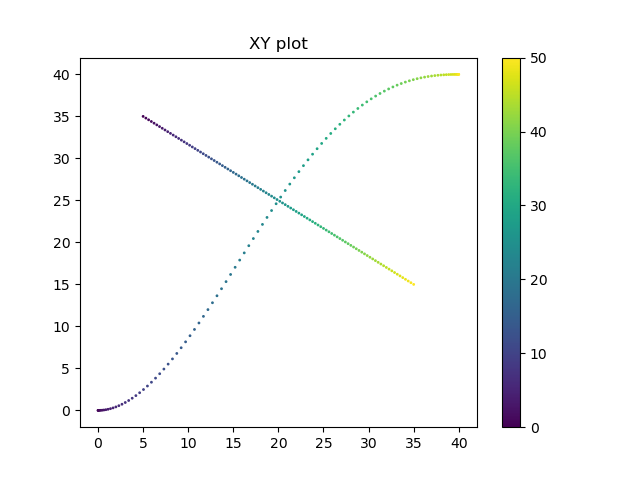
\includegraphics[width=\textwidth]{rb-cts-xy-plot.png}
        \caption{XY (time colormap)}
        \label{fig:sfig-rbcts-xy}
    \end{subfigure}
    \begin{subfigure}[b]{0.45\textwidth}
        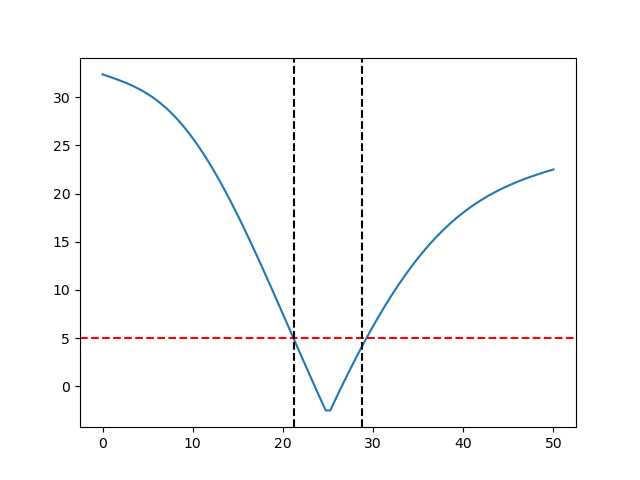
\includegraphics[width=\textwidth]{rb-cts-rule.png}
        \caption{Distance Rule}
        \label{fig:sfig-rbcts-rule}
    \end{subfigure}
    \caption{Rule-based constant time-scaling}
    \label{fig:rb-cts-exp1}
    The simulation is available as \texttt{rb\_cts\_exp1.avi} in the \href{https://iiitaphyd-my.sharepoint.com/:f:/g/personal/avneesh_mishra_research_iiit_ac_in/Er_wRqK4hxVLjVdL56rfDxYBKr9PPed1laN48hLgLisf4w}{shared OneDrive folder}. For figure \ref{sub@fig:sfig-rbcts-xy}, we see \texttt{XY} plot (colormap has time encoded). For figure \ref{sub@fig:sfig-rbcts-rule}, the distance is the line in blue (as time goes). The horizontal red line is a distance threshold. The two vertical lines indicate the start and end of time scaling (manually configured).
\end{figure}

\subsubsection*{Problems with Rule-based CTS}

The problems with \emph{rule-based} constant time scaling are mentioned below

\begin{itemize}
    \item The velocity profile, though being continuous, is \textbf{not} smooth. This leads to \emph{discontinuity in acceleration}, and this occurs at two places (starting and ending of time scaling). This leads to jerks in the motion. We could apply a variable time-scaling which smoothly varies the velocity profile, while keeping us on track.
    \item We could be \emph{wasting time} even after the collision point has passed. This can be mitigated by using a half-time window (than the actual one) from start to end. However, this assumes that the convergence and divergence patterns of the obstacle and robot are symmetric. If the obstacle takes long to diverge, then this could be risky.
\end{itemize}
